\documentclass[a4paper, 11pt]{article}
\usepackage[czech]{babel}
\usepackage[total={17cm, 24cm}, left=2cm, top=3cm]{geometry}
\usepackage[T1]{fontenc}
\usepackage[utf8]{inputenc}
\usepackage{times}
\usepackage{multirow}
\usepackage[linesnumbered, ruled, czech]{algorithm2e}
\SetKwFor{For}{for}{do}{end\ for}
\usepackage{amsmath}
\usepackage{graphicx}
\usepackage{float}
\usepackage{pdflscape}
\usepackage{picture}

\begin{document}
\catcode`\-=12
\begin{titlepage}
    \pagenumbering{gobble}
    
    \begin{center}
        \Huge
        \textsc{Vysoké učení technické v Brně}\\
        \huge
        \textsc{Fakulta informačních technologií\\}
        \vspace{0.382\textheight}
        \huge
        Typografie a publikování -- 2. projekt\\
        \Huge{Tabulky a obrázky}
        \vfill
        {\LARGE \today \hfill Josef Michal}
    \end{center}
    
\end{titlepage}
\pagenumbering{arabic}



\section{Úvodní strana}
Název práce umístěte do zlatého řezu a nezapomeňte uvést dnešní (today) datum a vaše jméno a příjmení.



\section{Tabulky}
Pro sázení tabulek můžeme použít buď prostředí tabbing nebo prostředí tabular.



\subsection{Prostředí\texttt{ tabbing}}
Při použití \texttt{tabbing} vypadá tabulka následovně:
\begin{tabbing}
    Vodní melouny\quad \= Množství\quad \= Jednotka\quad \= Cena za jedn.\quad \= \kill
    \textbf{Ovoce} \> \textbf{Množství} \> \textbf{Jednotka} \> \textbf{Cena za jedn.} \> \textbf{Cena celková}\\
    Jablka \> 3 \> kg \> 25,90\,kč \> 77,70\,kč\\
    Hrušky \> 2,5 \> kg \> 27,40\,kč \> 68,50\,kč\\
    Vodní melouny \> 1 \> kus \> 35,--\,kč \> 35,--\,kč\\
\end{tabbing}
Toto prostředí se dá také použít pro sázení algoritmů, ovšem vhodnější je použít prostředí\texttt{ algorithm }nebo \texttt{algorithm2e} (viz sekce \ref{sec:algo}).

\subsection{Prostředí\texttt{ tabular}}
Další možností, jak vytvořit tabulku, je použít prostředí tabular. Tabulky pak budou vypadat takto\footnote{Kdyby byl problém s cline, zkuste se podívat třeba sem: http://www.abclinuxu.cz/tex/poradna/show/325037.}:


\begin{table}[h]
\label{tab:mena}
\begin{center}
\begin{tabular}{| c | c | c |}\hline
    \multirow{2}{*}{\textbf{Měna}} & \multicolumn{2}{| c |}{\textbf{Cena}}\\\cline{2-3}
    & \textbf{nákup} & \textbf{prodej}\\\hline
    EUR & 23,26 & 24,93 \\\hline
    GBP & 29,56 & 29,83 \\\hline
    USD & 22,27 & 23,12 \\\hline
\end{tabular}
\caption{Tabulka kurzů k dnešnímu dni}
\end{center}
\end{table}
\bigskip

\begin{table}[h]
\label{tab:logical}
\begin{tabular}{| c | c |}\hline
    \emph{A} & \emph{\textlnot A}\\\hline
    \textbf{P} & N\\\hline
    \textbf{O} & O\\\hline
    \textbf{X} & X\\\hline
    \textbf{N} & P\\\hline
\end{tabular}
\begin{tabular}{| c | c | c | c | c | c |}\hline
  \multicolumn{2}{|c|}{\multirow{2}{*}{$A \wedge B$}} & \multicolumn{4}{c|}{\emph{B}} \\ 
  \cline{3-6}
  \multicolumn{2}{| c |}{} & \textbf{P} & \textbf{O} & \textbf{X} & \textbf{N} \\ \hline
  \multirow{4}{*}{\emph{A}} 
  & \textbf{P} & P & O & X & N \\ \cline{2-6}
  & \textbf{O} & O & O & N & N \\ \cline{2-6}
  & \textbf{X} & X & N & X & N \\ \cline{2-6}
  & \textbf{N} & N & N & N & N \\ \hline
\end{tabular}
\begin{tabular}{| c | c | c | c | c | c |}\hline
  \multicolumn{2}{|c|}{\multirow{2}{*}{$A \vee B$}} & \multicolumn{4}{c|}{\emph{B}} \\ 
  \cline{3-6}
  \multicolumn{2}{| c |}{} & \textbf{P} & \textbf{O} & \textbf{X} & \textbf{N} \\ \hline
  \multirow{4}{*}{\emph{A}} 
  & \textbf{P} & P & P & P & P \\ \cline{2-6}
  & \textbf{O} & P & O & P & O \\ \cline{2-6}
  & \textbf{X} & P & P & X & X \\ \cline{2-6}
  & \textbf{N} & P & O & X & N \\ \hline
\end{tabular}
\begin{tabular}{| c | c | c | c | c | c |}\hline
  \multicolumn{2}{|c|}{\multirow{2}{*}{$A \rightarrow B$}} & \multicolumn{4}{c|}{\emph{B}} \\ 
  \cline{3-6}
  \multicolumn{2}{| c |}{} & \textbf{P} & \textbf{O} & \textbf{X} & \textbf{N} \\ \hline
  \multirow{4}{*}{\emph{A}} 
  & \textbf{P} & P & O & X & N \\ \cline{2-6}
  & \textbf{O} & P & O & P & O \\ \cline{2-6}
  & \textbf{X} & P & P & X & X \\ \cline{2-6}
  & \textbf{N} & P & P & P & P \\ \hline
\end{tabular}
\caption{Protože Kleeneho trojhodnotová logika už je ”zastaralá“, uvádíme si zde příklad čtyřhodnotové logiky}
\end{table}
\clearpage

\section{Algoritmy}
\label{sec:algo}
Pokud budeme chtít vysázet algoritmus, můžeme použít prostředí \texttt{algorithm2\footnote{http://ftp.cstug.cz/pub/tex/CTAN/macros/latex/contrib/algorithms/algorithms.pdf}} nebo \texttt{algorithm2e3\footnote{http://ftp.cstug.cz/pub/tex/CTAN/macros/latex/contrib/algorithm2e/doc/algorithm2e.pdf}}. 
Příklad použití prostředí \texttt{algorithm2e} viz Algoritmus \ref{alg:fastslam}.

\SetAlgoNoLine
\SetNlSty{}{}{:}
\begin{algorithm}[h]
\caption{FastSLAM}
\label{alg:fastslam}
\DontPrintSemicolon
\Indm
\KwIn{($X_{t-1}, u_t, z_t$)}
\KwOut{$X_t$}
\Indp

$\overline{X_{t}} = X_{t} = 0 $\;
\For{$k = 1$ \KwTo $M$}{
    $x_{t}^{[k]} = \text{sample\_motion\_model}(u_{t}, x_{t-1}^{[k]})$\;
    $\omega_t^{[k]} = \text{measurement\_model}(z_{t}, x_{t}^{[k]}, m_{t-1})$\;
    $m_{t}^{[k]} = \text{updated\_occupancy\_grid}(z_{t}, x_{t}^{[k]}, m_{t-1}^{[k]})$\;
    $\overline{X} = \overline{X} + \langle x_x^{[m]}, \, \omega_{t}^{[m]}\rangle$\;
}
\For{$k = 1$ \KwTo $M$}{
    $\text{draw \textit{i} with probability} \approx \omega_t^{[i]}$\;
    $\text{add } \langle x_{x}^{[k]}, m_{t}^{[k]} \rangle \text{ to } X_{t}$\;
}
\Return $X_{t}$\;   % The final line can be a "return"

\end{algorithm}

\section{Obrázky}
Do našich článků můžeme samozřejmě vkládat obrázky. Pokud je obrázkem fotografie, můžeme klidně použít
bitmapový soubor. Pokud by to ale mělo být nějaké schéma nebo něco podobného, je dobrým zvykem takovýto
obrázek vytvořit vektorově.
\begin{figure}[h]
\label{pic:etiopanci}
\centering
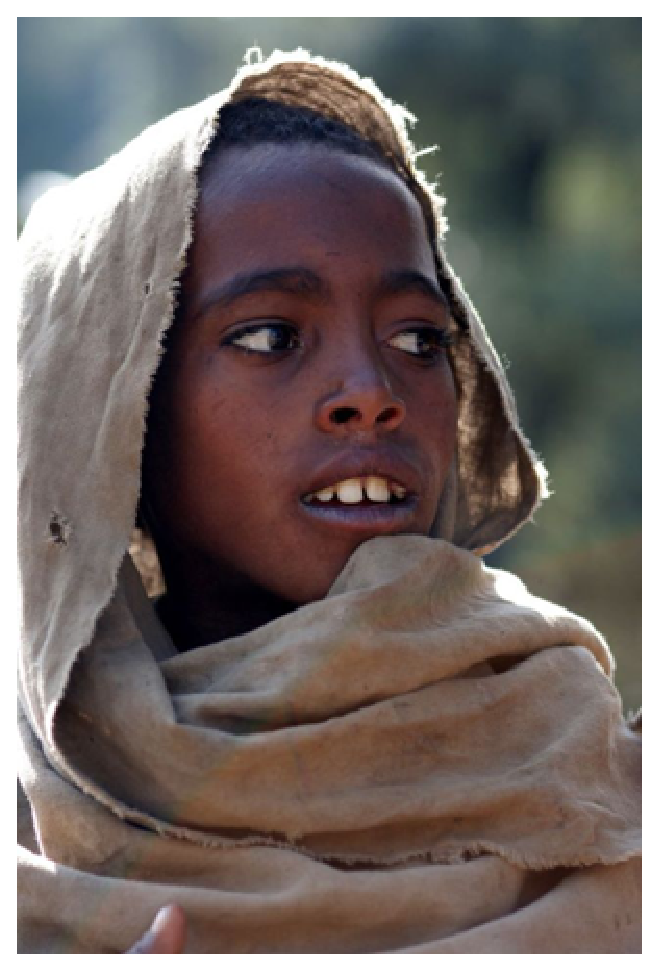
\includegraphics[width=0.25\textwidth]{etiopan.eps}
\reflectbox{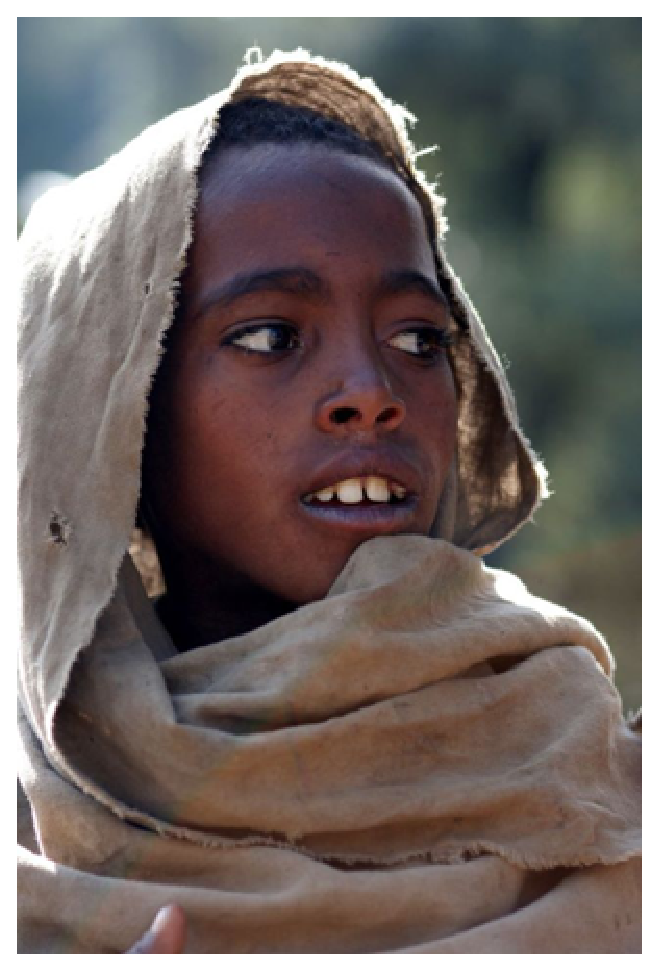
\includegraphics[width=0.25\textwidth]{etiopan.eps}}
\caption{Malý Etiopánek a jeho bratříček}
\label{fig:etiopan}
\end{figure}
\clearpage
Rozdíl mezi vektorovým\dots
\begin{figure}[H]
\label{pic:vector}
\centering

\includegraphics[width=0.5\textwidth]{oniisan.eps}
\caption{Vektorový obrázek}
\label{fig:oniisan1}
\end{figure}
\noindent \dots a bitmapovým obrázkem
\begin{figure}[H]
\label{pic:bitmap}
\centering

\includegraphics[width=0.5\textwidth]{oniisan2.eps}
\caption{Bitmapový obrázek}
\label{fig:oniisan2}
\end{figure} 
\noindent se projeví například při zvětšení.

Odkazy (nejen ty) na obrázky 1, 2 a 3, na tabulky 1 a 2 a také na algoritmus 1 jsou udělány pomocí křížových 
odkazů. Pak je ovšem potřeba zdrojový soubor přeložit dvakrát.

Vektorové obrázky lze vytvořit i přímo v \LaTeX u, například pomocí prostředí \texttt{picture}.

\clearpage

\begin{landscape}
\begin{figure}
\label{pic:house}
\begin{picture}(200, 200)(-100, 100) %Dum neni hotovy, ale ma pripominat: https://maps.app.goo.gl/eLcHEegaxZ2PfseLA

    \put(0, 0){\framebox(150, 300){}}
    \put(150, 300){\line(2, -5){20}}
    \put(170, 250){\line(0, -1){250}}
    
    \qbezier(30, 250)(45, 270)(60, 250) %left window
    
    \put(30, 250){\line(0, -1){40}} %window verticals
    \put(45, 260){\line(0, -1){50}}
    \put(60, 250){\line(0, -1){40}}
    
    \put(30, 250){\line(1, 0){30}} %window horizontals
    \put(30, 245){\line(1, 0){30}}
    \put(30, 210){\line(1, 0){30}}
    
    \qbezier(70, 250)(85, 270)(100, 250) %right window
    
    \put(70, 250){\line(0, -1){40}}
    \put(85, 260){\line(0, -1){50}}
    \put(100, 250){\line(0, -1){40}}

    \put(70, 250){\line(1, 0){30}}
    \put(70, 245){\line(1, 0){30}}
    \put(70, 210){\line(1, 0){30}}

    \put(45, 50){\line(0, 1){65}} %bottom window
    \put(85, 50){\line(0, 1){65}}
    \put(65, 50){\line(0, 1){65}}
    
    \put(45, 50){\line(1, 0){40}}
    \put(45, 88){\line(1, 0){40}}
    \put(45, 92){\line(1, 0){40}}
    \put(45, 115){\line(1, 0){40}}

    \put(0, 300){\line(1, 1){40}} %roof
    \put(40, 340){\line(2, 1){20}}
    \put(60, 350){\line(1, 0){140}}

    \put(150, 300){\line(1, 1){70}}
    \put(220, 370){\line(1, -1){70}}
    \put(290, 300){\line(0, -1){300}}

    \put(150, 0){\line(1, 0){140}}

    \put(130, 340){\line(0, 1){40}}
\end{picture}
\caption{Vektorový obrázek moderního bydlení vhodného pro 21. století}
\end{figure}
\end{landscape}

\end{document}
